\subsection*{Question 2.4}

For the shared covariances of the maximum likelihood problem, gives a
linear classifications, as it can be seen in
figure \ref{fig:q24a}. For the independent covariances, the
classification is non-linear, ant it splits op in are split green
class, as can be seen in figure
\ref{fig:q24b}, this cut be are case of over fitting. In comparison to
the optimal decision regions, figure \ref{fig:q24a} compares best and is
the classification model that fits best.

\begin{figure}[!htbp]
  \centering
  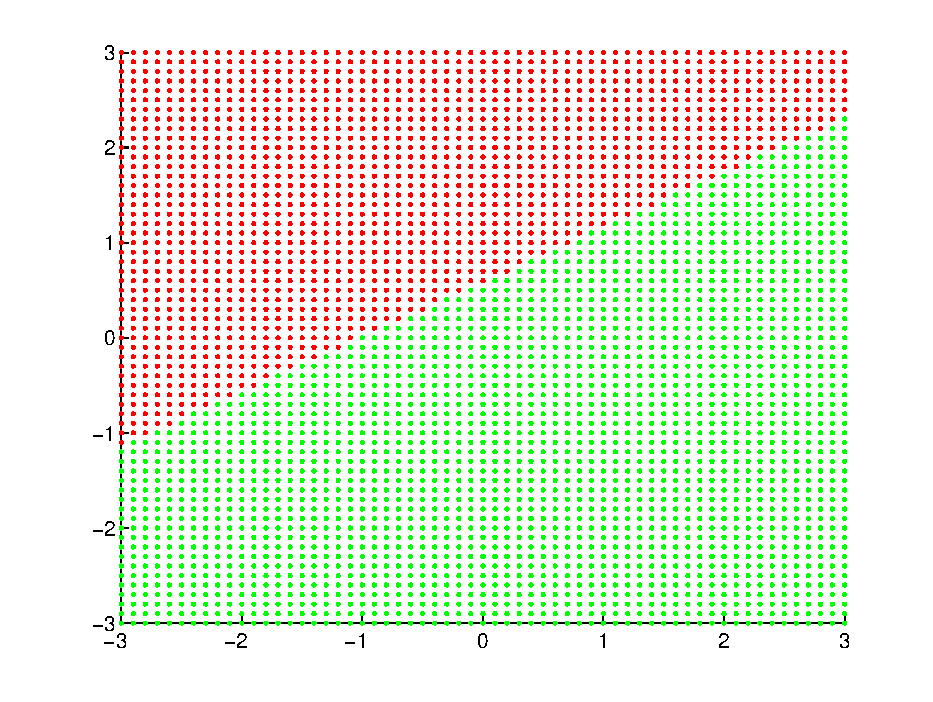
\includegraphics[width=0.6\textwidth]{./images/q24a.pdf}
  \caption{Shared covariance, $N1 = 50$, $N2= 200$}
  \label{fig:q24a}
\end{figure}

\begin{figure}[!htbp]
  \centering
  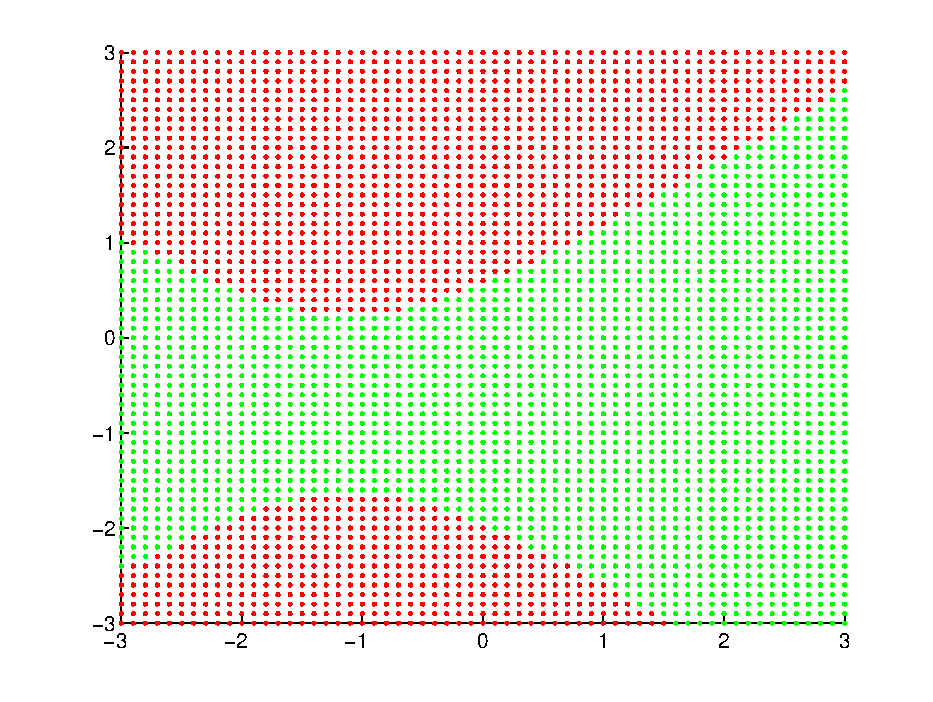
\includegraphics[width=0.6\textwidth]{./images/q24b.pdf}
  \caption{Independent covariance, $N1 = 50$, $N2= 200$}
  \label{fig:q24b}
\end{figure}
